\chapter{Introduction}
\todo{why are there spaces?}
The rising popularity of video games has transformed them from niche entertainment into a mainstream medium. As a result, game development has attracted a diverse audience, including enthusiasts with limited programming experience. To meet the growing demand for accessible game development tools, various frameworks and platforms have been developed. Their goal is to simplify the creation process, helping developers bring their visions to life without requiring extensive coding expertise.

One genre that holds a special place in gaming history is point-and-click adventure, which emerged in the early 1980s and continues to influence the industry to this day. Despite its seemingly straightforward gameplay, creating a point-and-click adventure game involves implementing complex systems, such as a walking system, inventory mechanics, dialogue trees, and puzzle design. For novice developers, replicating these systems can be significantly difficult.

The goal of this Bachelor thesis is to design and implement a framework in the Unity game engine tailored to the development of 2D point-and-click adventure games. This framework will prioritize functionality, user-friendliness, and accessibility, encouraging beginner to intermediate game developers to create engaging games without requiring advanced programming knowledge. By addressing the unique challenges associated with point-and-click adventure game development, this thesis seeks to provide a valuable tool for aspiring developers, encouraging innovation in this beloved genre.

\section{Point-and-click adventure games}
\subsection{Definition}
A point-and-click adventure game is a type of interactive video game that emphasizes exploration, puzzle solving, and narrative engagement through a graphical user interface. This genre is characterized by their intuitive graphical user interface (GUI), which allows players to interact with rich environments through mouse-based controls. Players use a cursor to click on objects, locations, or characters within a visual scene to trigger actions or dialogues. These games emphasize narrative-driven gameplay, immersing players in stories often involving mystery, exploration, or character-driven plots. The progression typically involves solving puzzles, collecting and combining items, interpreting clues, and completing tasks in an environment. As the genre evolved, games started to implement simplified interaction systems such as clickable text buttons and action icons (e.g., 'look', 'take', or 'speak') which greatly improved accessibility. Some later titles took this concept even further by eliminating the need for players to choose between actions. Instead, the game selects the appropriate action based on the context and object with which the player interacts with like in \textit{Return to Monkey Island} (2022). Even typical point-and-click character controls are being replaced by direct controls using a joystick or keyboard in some modern games. There is also a tendency to include more action and fewer puzzles such as in titles developed by Telltale Games \cite{Carton2023history}. 


\subsection{History}
The emergence of point-and-click adventure games can be traced back to the 1960s, although the exact origins of the genre is challenging to determine. Early text-based video games like \textit{The Sumerian Game} (1964) introduced simple verb-noun parsers that allowed players to interact with the game world by typing commands. \cite{Salter2014}[p. 29]. Building on this foundation, a notable predecessor to the point-and-click genre \textit{Colossal Cave Adventure} (1976) and games directly inspired by its legacy like \textit{Mystery House} (1980) and \textit{The Hobbit} (1982) took the first steps toward integrating graphics into adventure gameplay. These games, while still reliant on text-based commands, incorporated static visuals to represent the game world, marking a significant departure from the purely text-driven interfaces of earlier adventure titles. The next stage of evolution introduced animated visuals and greater graphical complexity which allowed players to manipulate an avatar directly. For example, in games influenced by \textit{Mystery House}, such as \textit{Valhalla} (1983) and \textit{King's quest} (1984), players could enter commands like 'go west' to move their avatar within the graphical environment \cite{Salter2014}[p. 38]. 

These developments paved the way for a big shift in interaction methods, as the inclusion of mouse technology transformed gameplay. The screens became clickable, allowing players to point to places or objects in the environment to interact with them. So, the typed commands were replaced with more intuitive and immediate actions.


\begin{figure}[H]
\centering
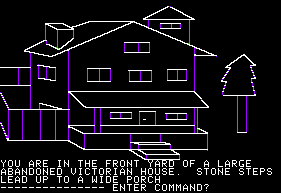
\includegraphics{img/Mystery_House.png}
\caption{The opening scene from Mystery House (1980). Source: https://commons.wikimedia.org\cite{wiki:MysteryHouse}}
\label{fig:MH}
\end{figure}

This is where the contenders for the title of the first point-and-click adventure game come into the scene, among those \textit{Enchanted Scepters}. For many years, this game was believed to have debuted in 1984. However, later investigations revealed that its release likely occurred later, in November 1985. This revelation has shifted the discussion to \textit{Deja Vu: A Nightmare Begins}, released at least a month earlier. Now this game emerges as a leading candidate for the first true point-and-click adventure game\cite{Pfenning2024}.

Point-and-click adventure games experienced their golden age in the late 1980s and early 1990s, with iconic titles such as \textit{The Secret of Monkey Island} (1990), \textit{Beneath a Steel Sky} (1994), and \textit{Myst} (1994) captivating players with their innovative storytelling and puzzle-solving gameplay. However, as the decade progressed, the popularity of the genre slowed down\cite{Qaffas202022} with fewer mainstream releases and a shift to more niche titles such as the \textit{Nancy Drew} game series.

In recent years, the point-and-click adventure genre has undergone a renaissance. Modern titles such as \textit{Thimbleweed Park} (2017) and \textit{Return to Monkey Island} (2022) have revived interest by paying homage to the retro roots of the genre while implementing modern design elements. This resurgence has also been fueled by the cinematic storytelling approach pioneered by \textit{Telltale Games}, whose narrative-driven series brought the genre back into the mainstream spotlight.

The renewed interest in point-and-click adventure games highlights their timeless appeal and presents an opportunity for new developers to explore the genre. Building on its rich legacy, aspiring game creators can reimagine and modernize these games for today's audience. This cultural revival highlights the need for accessible development tools to support and sustain the creative evolution of this genre.

\section{Common features}
\todo{Different title?}
So far in this chapter, we have introduced point-and-click adventure games to highlight their importance as a game genre. Now we will take a look at concrete examples of 2D point-and-click adventure games and specifically their prominent features and characteristics that could inspire us in the design and creation of the final work.

\subsection{The Secret of Monkey Island (1990)}
Released in 1990 by Lucasfilm Games, The Secret of Monkey Island is a 2D point-and-click graphic adventure game set in the Caribbean. Our main protagonist is Guybrush Threepwood, an aspiring pirate who embarks on his quest to achieve his dream.

One of the main ways players can engage with the world is the action panel, which is typical of games from that era, as seen in Figure \ref{fig:TSoMI}. These \textit{panel actions} are very contextual--if you select a panel action and hover over an object, a short sentence will be created in the upper part of the panel to give an indication to the player of what the main character is going to do. In Figure \ref{fig:TSoMI}, the panel action 'Look at' is selected, and then the mouse cursor is placed over a table. This sequence of actions creates the sentence 'Look at table'. By following this logic, longer sentences can be obtained.

For each object in the game, there is a limited number of panel actions that have a meaningful result. Those that do not make sense for the given object result in the straightforward answer something along the lines of 'I cannot [insert panel action] this.' Then there are some that result in a humorous response but do not help to progress the story. And finally, certain panel actions help you obtain a piece of information (the panel action 'Look at'), change the state of an object (the panel actions 'Open', 'Push', etc.), let you talk to an NPC (the panel action 'Talk to'), or let you obtain or remove an item from player's inventory (the panel actions 'Pick up' and 'Give').

\begin{figure}[H]
\centering
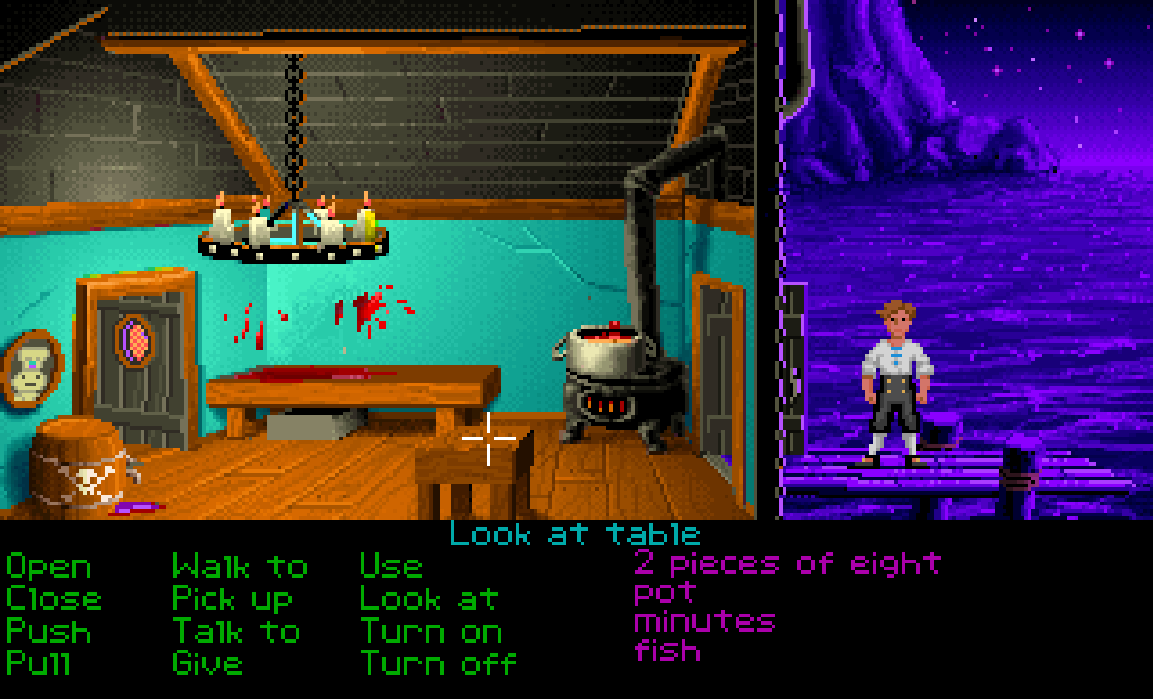
\includegraphics[width=1.\linewidth]{img/TSoMI.png}
\caption{The protagonist Guybrush Threepwood is standing on the dock. In the lower part of the image there is a panel with various actions (\textit{panel actions}) such as 'Open', 'Look at', and 'Use' to interact with the environment. The  panel also includes a list of items in player's inventory. Player's mouse cursor is hovering over a table.}
\label{fig:TSoMI}
\end{figure}

The main character's movement is managed through mouse clicking, a common method in 2D point-and-click games from this era. Other notable features of the game include puzzles, cutscenes, and dialogue trees. To talk to NPCs, the player must first enter the dialogue mode by selecting the 'Talk to' panel action and afterwards clicking on an them. When done so, some features, such as the inventory, are inaccessible. Instead, the player can choose an option on how to respond to an NPC. By selecting a specific option, the dialogue mode ends, and the player is back in gameplay mode.

\subsection{Beneath a Steel Sky (1994)}
Developed by the British studio Revolution Software and launched in 1994, Beneath a Steel Sky is a point-and-click adventure game set in a cyberpunk-inspired dystopian future. The players guide Robert Foster as he uncovers hidden secrets of this foreign world.

The game is primarily controlled by the mouse. If the player hovers the mouse cursor over an object, a short text will pop up describing what that object is.

When clicking with the right mouse button on an object, Foster will either pick it up or use it in some way (or talk to an NPC if that object was one). The game decides what the action will lead to.

The inventory in this game is slightly hidden. The player must move the mouse to the top of the screen to make the inventory panel slide down. Following this, the player can see the icons of all items in the inventory as well as their names when the mouse hovers over an icon. To see a longer description, the player has to click on the item with the left mouse button. If the player decides to use an item on an object, they must grab an icon using the right mouse button and then lead the item to the location of the object. This action is captured in Figure \ref{fig:BaSS}.

\todo{write how to talk to NPCs}

\begin{figure}[H]
\centering
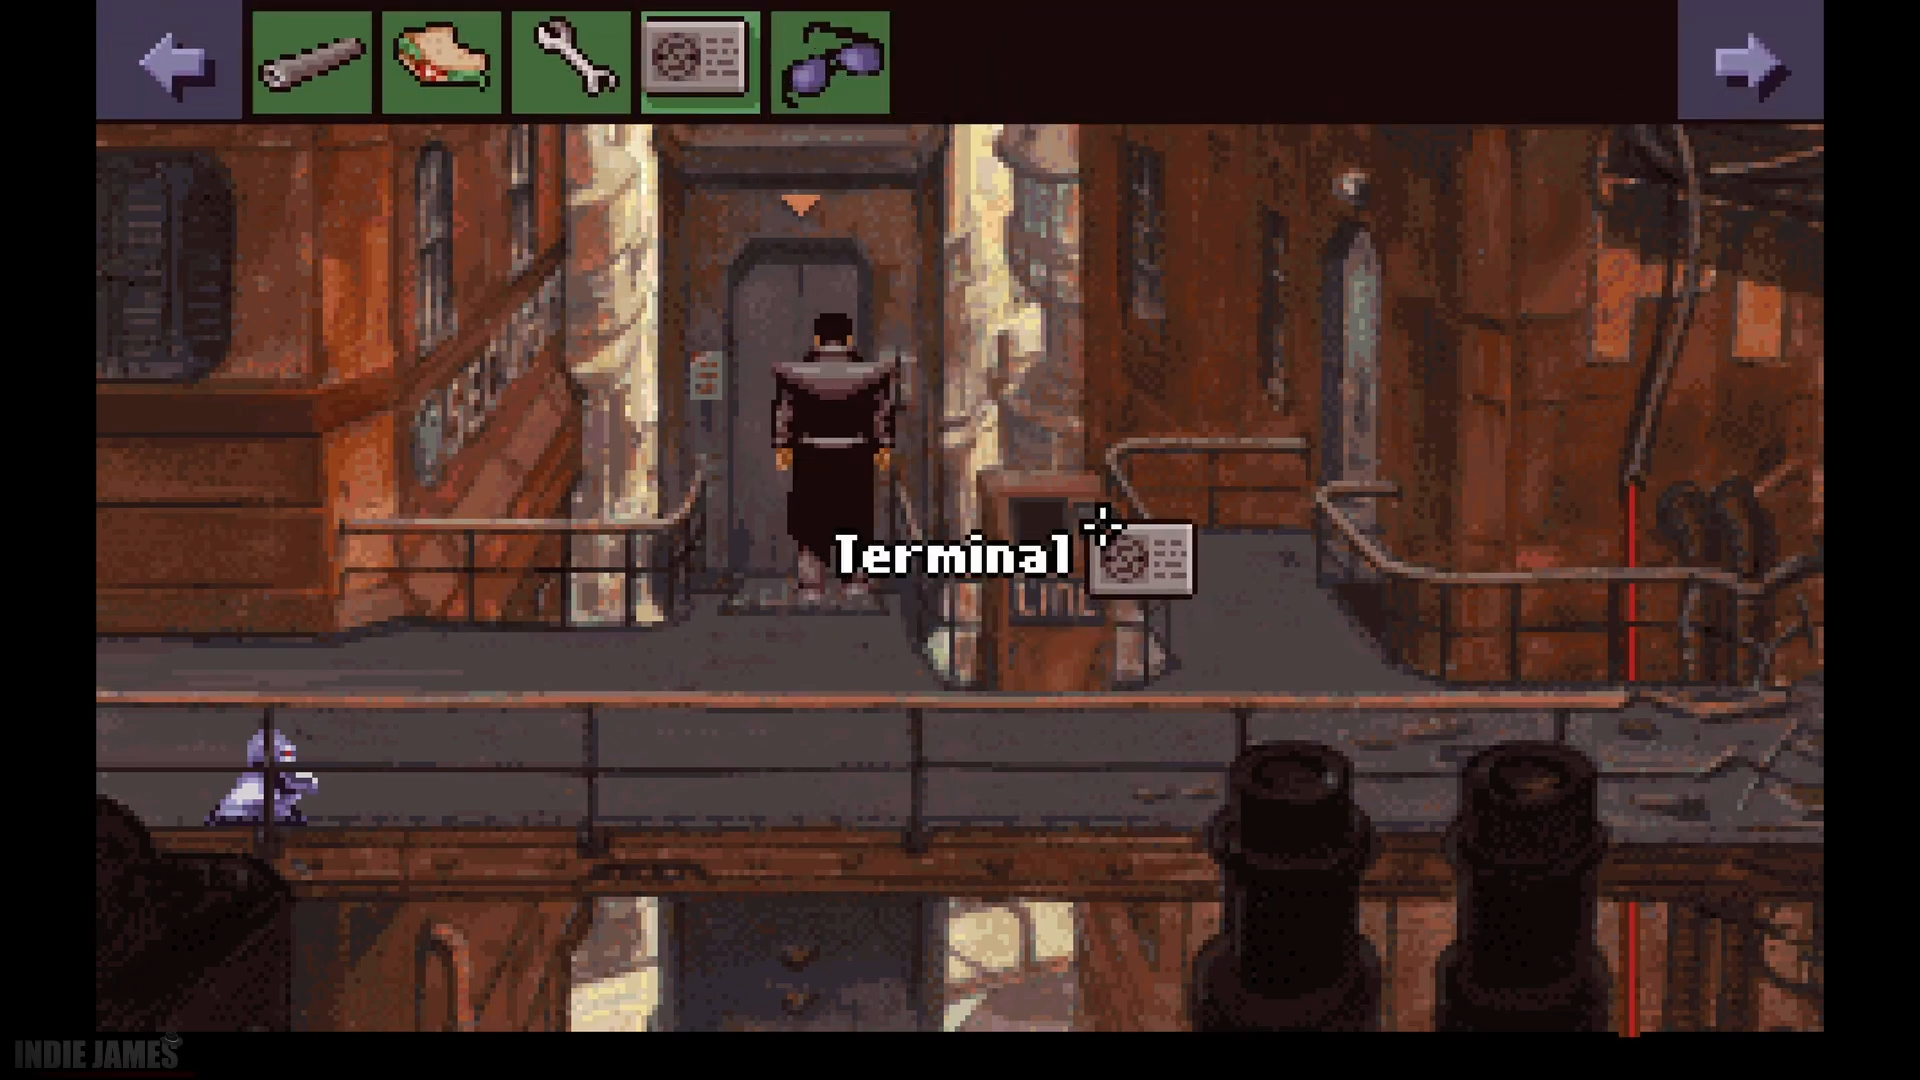
\includegraphics[width=1.\linewidth]{img/BaSS.png}
\caption{The protagonist Robert Foster is standing in front of an elevator. In the upper part of the image there is a panel with his inventory. A mouse cursor is located on an object (a terminal, to be precise) while holding an ID card from the inventory.}
\label{fig:BaSS}
\end{figure}

\subsection{Fran Bow (2015)}
Created by the Swedish indie studio Killmonday Games, Fran Bow is a 2D point-and-click adventure game with elements of psychological horror. The game is set in 1944 and it tells the story of Fran, a ten-year-old girl suffering from a mental illness after the death of her parents.

The inventory can be accessed by clicking on an icon of a purse in the lower left corner. A panel appears with everything the main character has with her. In addition to the panel, there are three buttons with different actions the player can take. When an item is selected and "Examine" is pressed, Fran Bow says something about the item. Next to it, there is a 'Combine' option which allows you to choose two items and create a new one in their place inside the inventory. Finally, the third button with the "Use" label is a bit more versatile. Depending on the item, the player can either inspect the item closer and interact with it (for example, unlocking a locked box and finding hidden items), or use the item outside of the inventory (for example, giving an item to an NPC).

In Figure \ref{fig:FranBow}, there is an inventory from game Fran Bow containing various items. The player is combining two items using the "Combine" button. At the bottom of the screen, there is a short sentence that describes exactly what the player is going to do.

\begin{figure}[H]
\centering
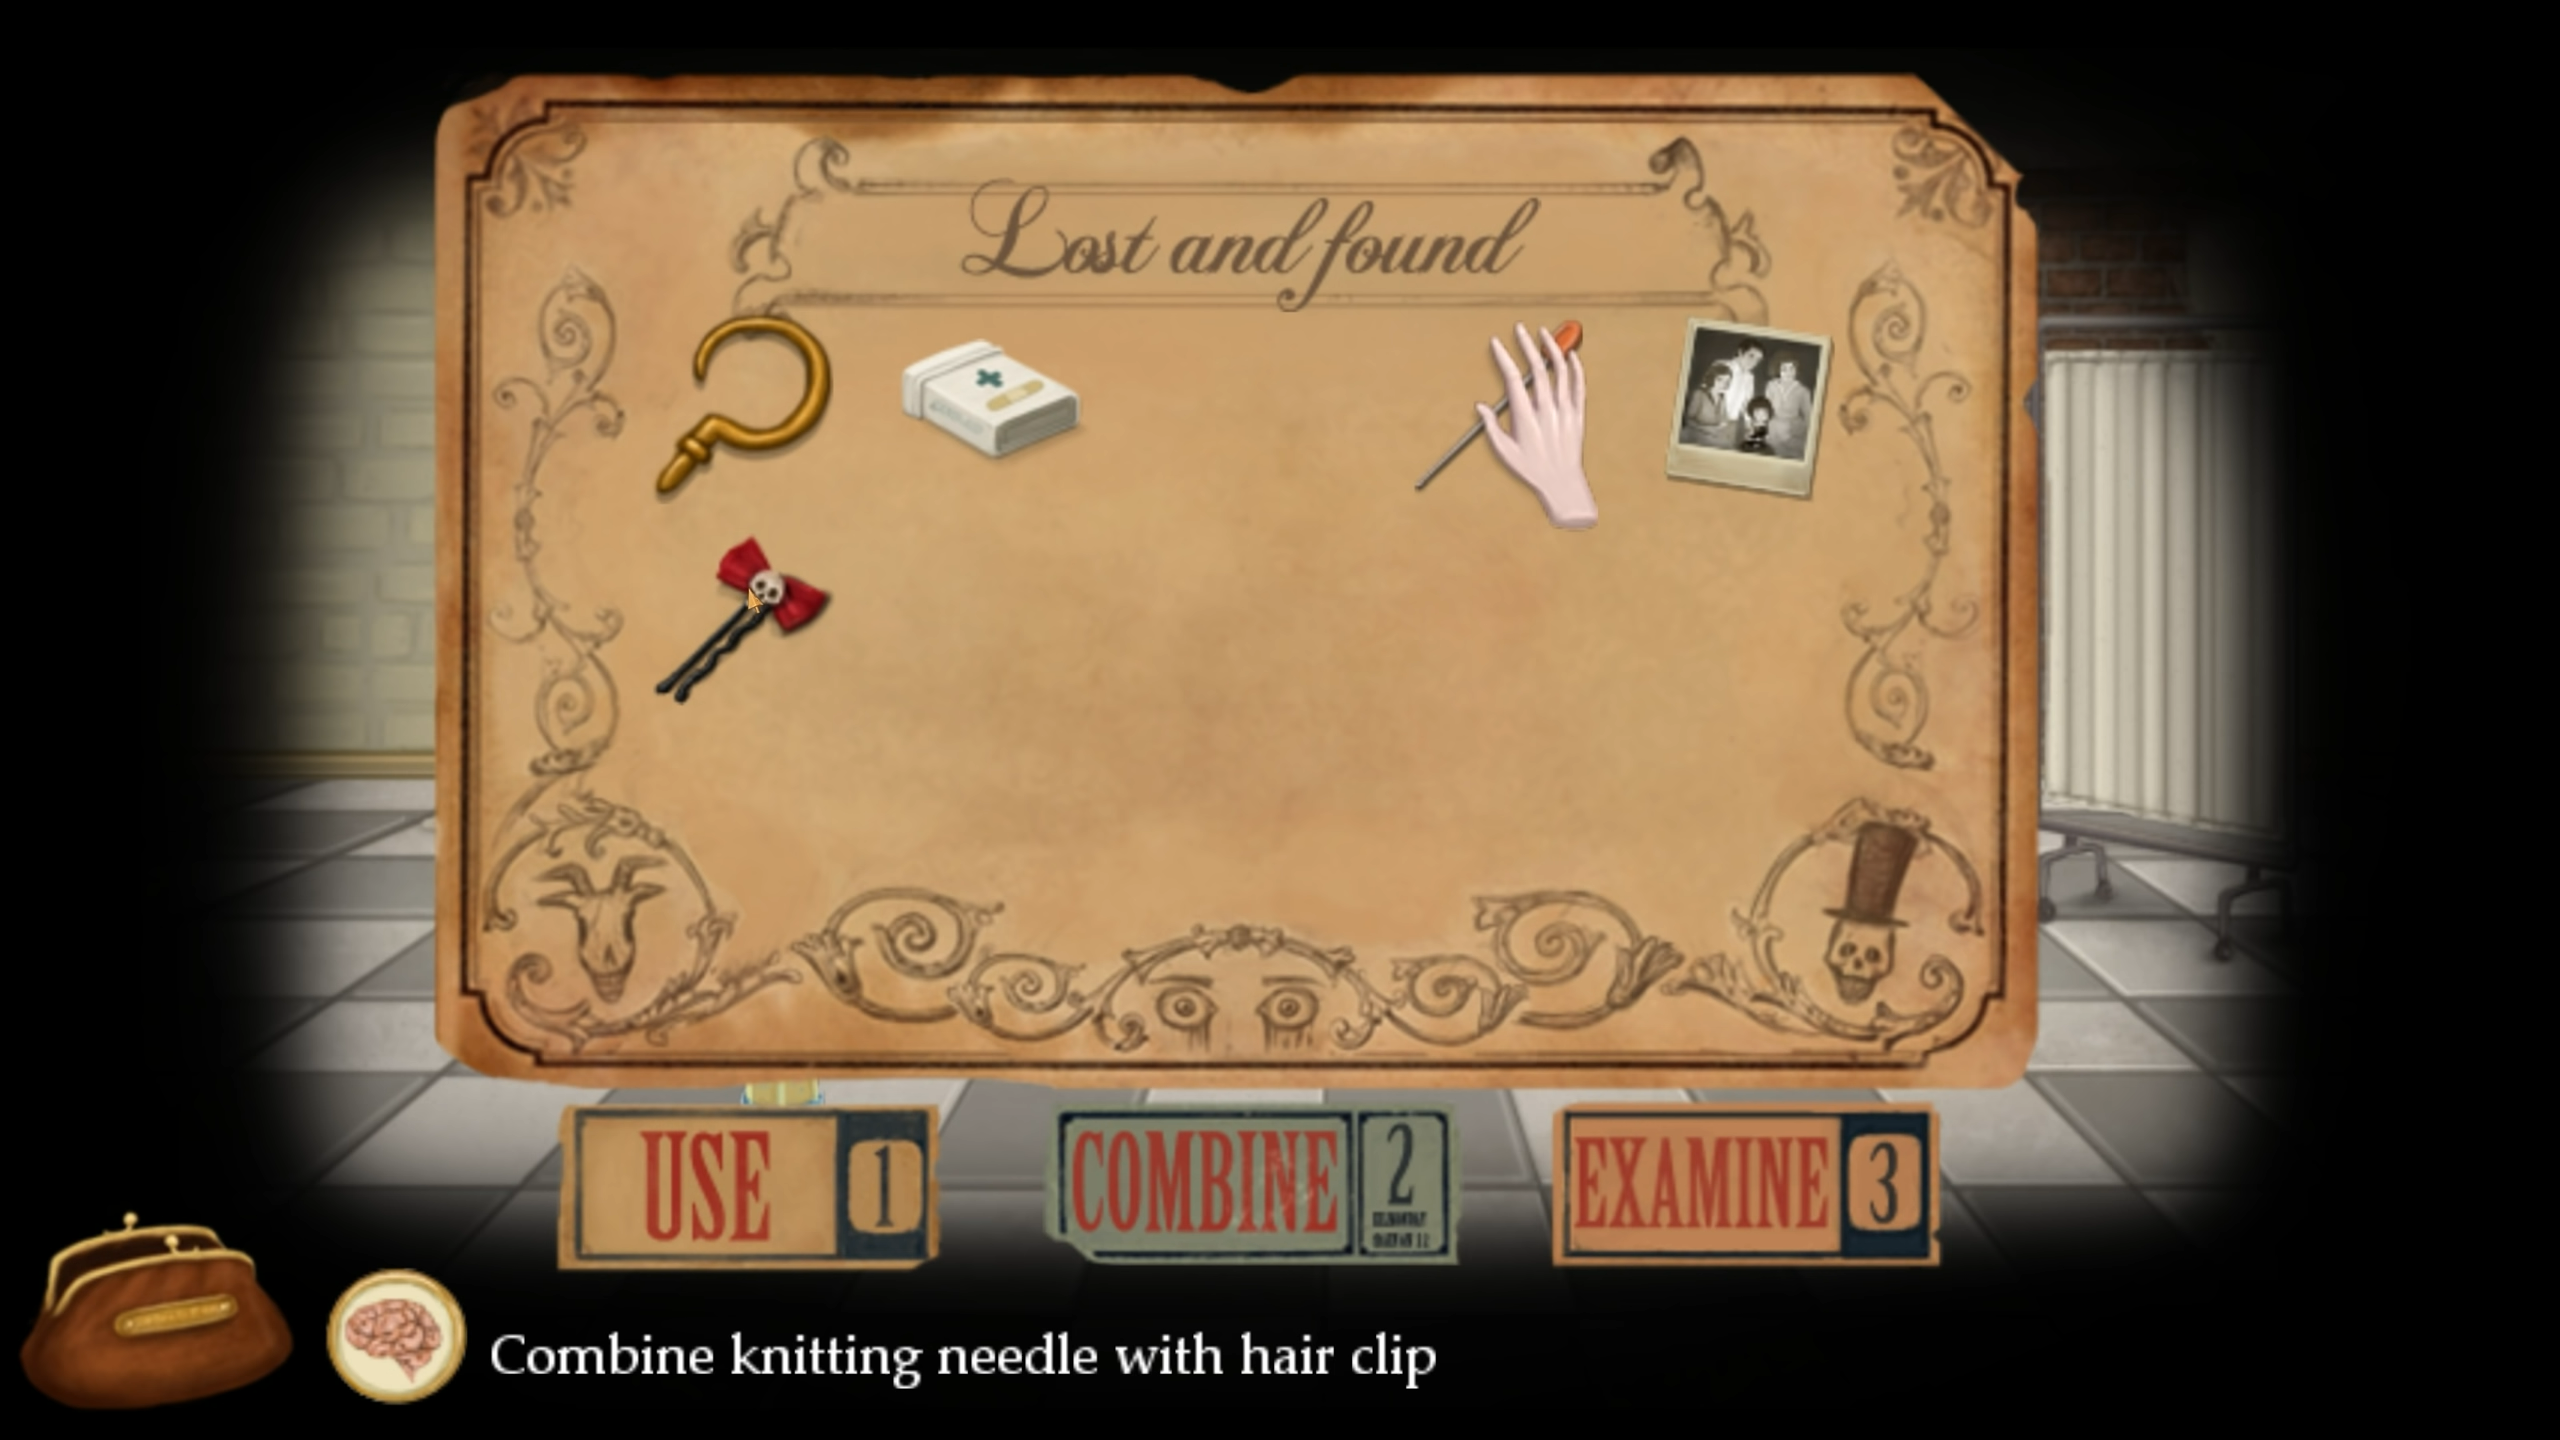
\includegraphics[width=1.\linewidth]{img/Fran_Bow.png}
\caption{The inventory for Fran Bow is accessed as a pop-up panel. It contains all items the player has collected. Below there are three action buttons for player to use. At the very bottom there is a sentence describing the action the player is going to take.}
\label{fig:FranBow}
\end{figure}

The main character's movement is also managed through mouse clicking. The game includes puzzles, cutscenes, and fairly straightforward dialogue trees.

\todo{write how to talk to NPCs}

\subsection{Thimbleweed Park (2017)}

Thimbleweed Park, developed by Terrible Toybox, serves as a spiritual successor to Maniac Mansion (1987) and The Secret of Monkey Island (1990) and is crafted to emulate the visual style and gameplay mechanics of graphic adventure titles from that era. Thimbleweed Park tells the intriguing story of two detectives brought in to investigate a mysterious body discovered in a river near the town. The players switch between five different characters as they enter the dark, satirical and eccentric world of Thimbleweed Park\cite{Matulef2014}.

\todo{write more describing the game}

\begin{figure}[H]
\centering
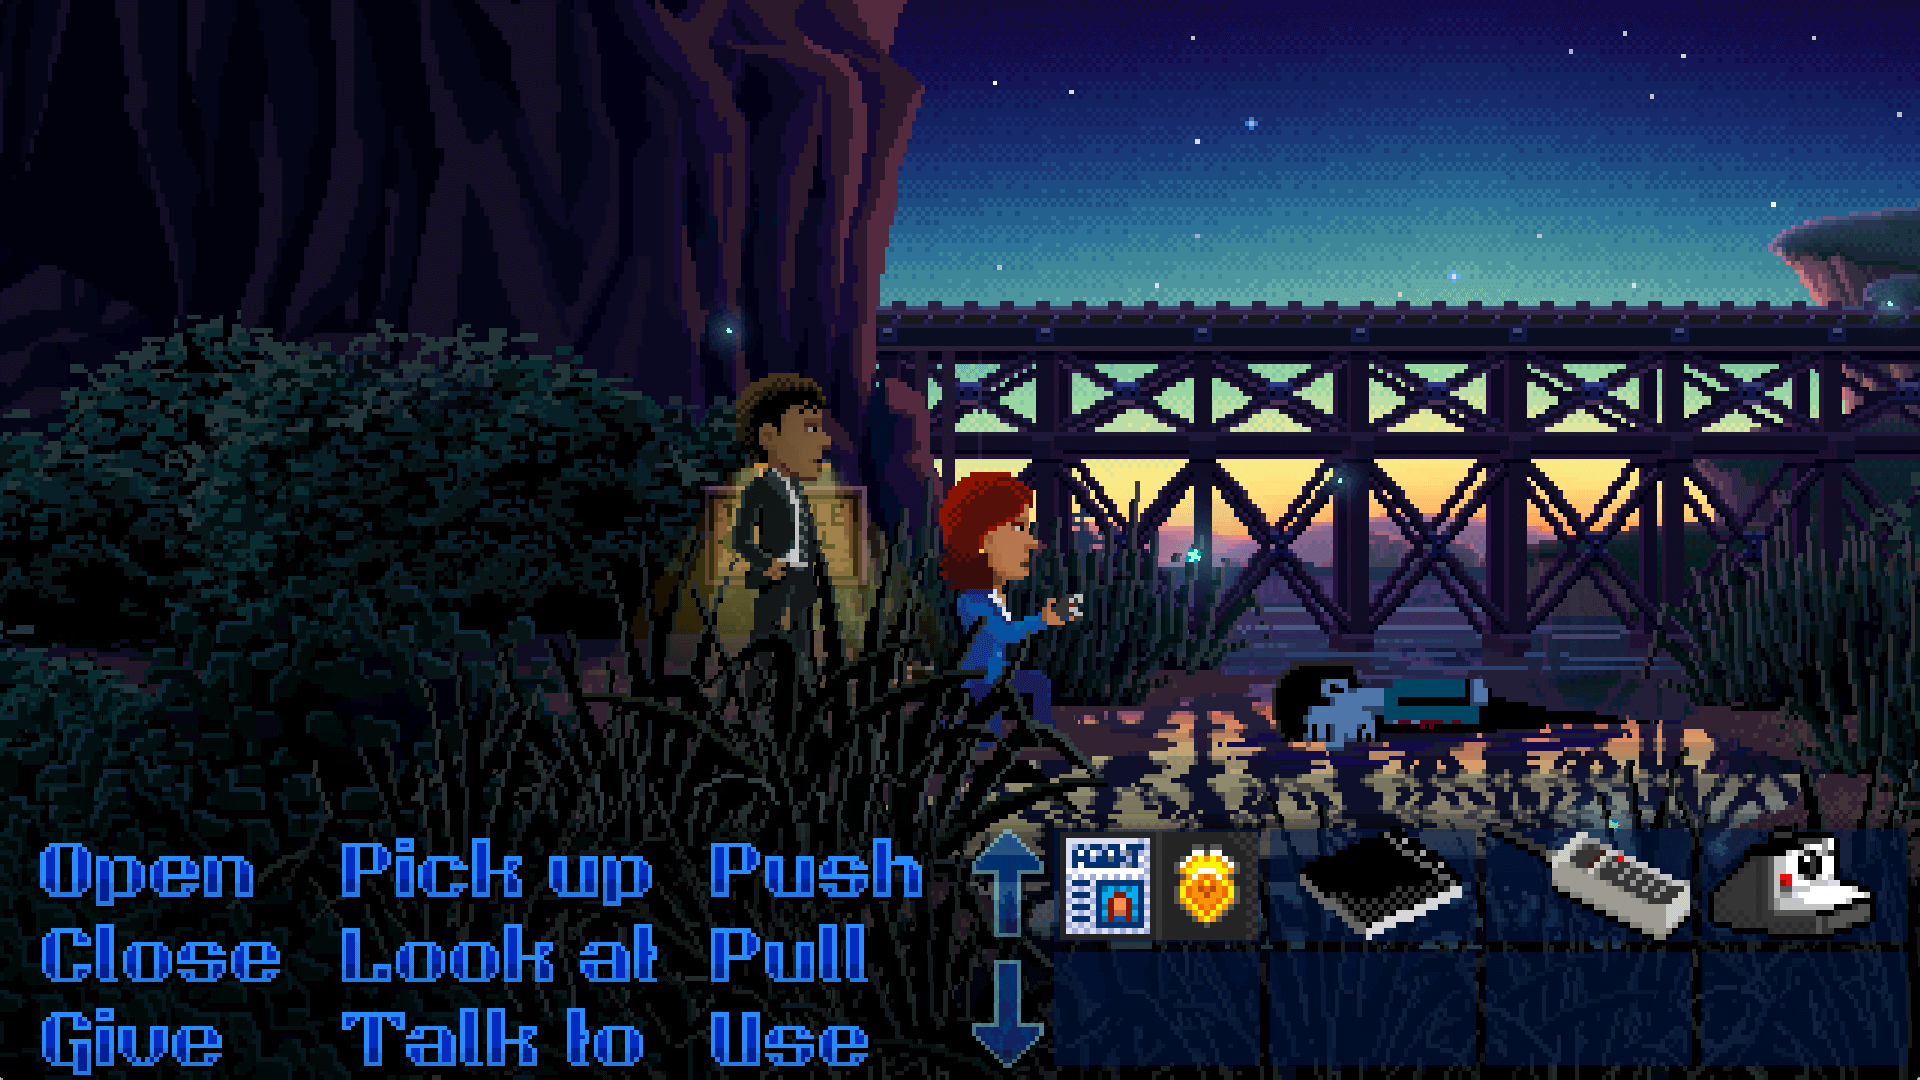
\includegraphics[width=1.\linewidth]{img/TWP.png}
\caption{The player is controlling one of the two FBI agents Angela Ray. She is squatting and taking a picture of a body. In the lower part of the image there is a panel with panel actions such as 'Open', 'Pick up', and 'Talk to'. It also includes a list of items in player's inventory. Its layout is very reminiscent of the one in Figure \ref{fig:TSoMI}. Source: https://store.epicgames.com \cite{epic:TWP}}
\label{fig:TWP}
\end{figure}

\subsection{Return to Monkey Island (2022)}

Return to Monkey Island, created by Terrible Toybox in collaboration with Lucasfilm Games, is a 2D point-and-click adventure game and the sixth entry in the Monkey Island series. The pirate Guybrush Threepwood returns once again to uncover the secret of Monkey Island\cite{McCaffrey2022}.

\todo{write more describing the game. also 0.7 for pics so that they fit on page}

\begin{figure}[H]
\centering
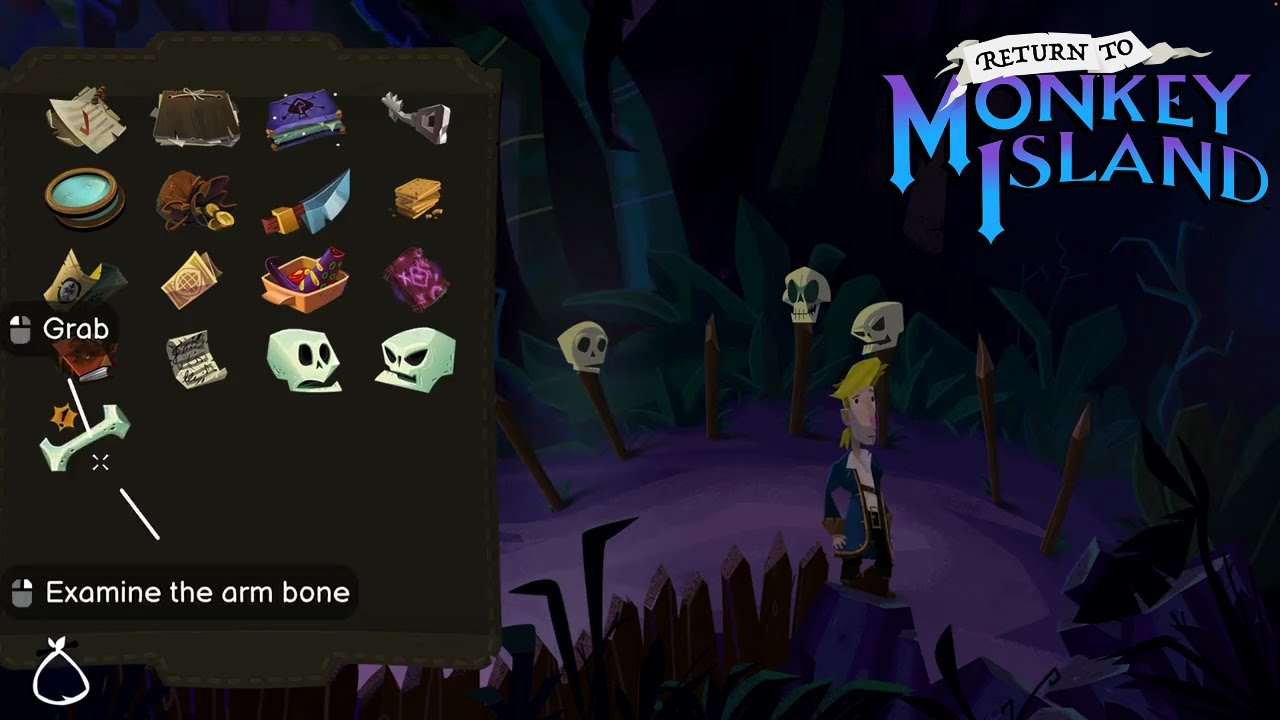
\includegraphics[width=.7\linewidth]{img/RtMI1.png}
\caption{Source:  \cite{}}
\label{fig:RtMI1}
\end{figure}

\begin{figure}[H]
\centering
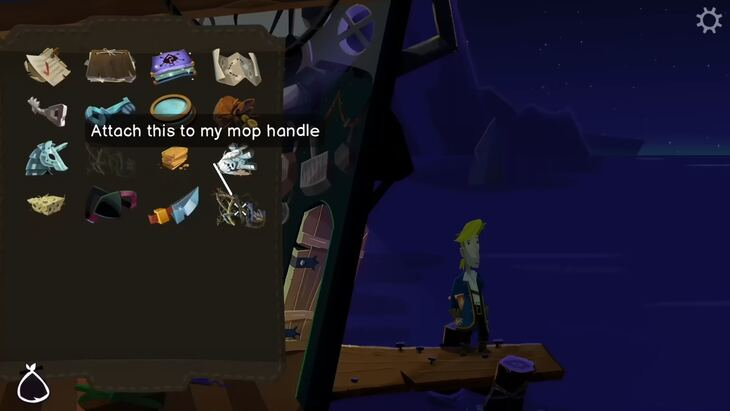
\includegraphics[width=.7\linewidth]{img/RtMI2.png}
\caption{Source:  \cite{}}
\label{fig:RtMI2}
\end{figure}

\section{Game specifications}

Now, since we looked at some examples of 2D point-and-click adventure games, we can examine their defining features and create an outline of our project. 

We will look closely at the following features.
\begin{itemize}
\item Inventory
\item Character movement
\item Actions
\item Dialogue
\end{itemize}

\subsection{Inventory}
There is a great variety of types of inventories as seen in the examples. Typically, it is a panel that contains icons or names of items that the player had collected on their journey. The panel might be hidden (like in Beneath the Steel Sky, Fran Bow and Return to Monkey Island) or revealed throughout the whole game (The Secret of Monkey Island and Thimbleweed Park). In all games, the player can use the items in the environment. There is also an option to combine two items to create another or to examine them more closely. Every game deals with it a bit differently... \todo{continue}
I will try to take all of this into account and create an inventory system that satisfies these needs.

\subsection{Character movement}
A typical method of movement control is clicking on a part of the environment using a mouse or another input method and waiting for the character to get to the point themselves. From the games I have selected, none of them uses another input method \todo{need to check for sure or maybe choose a game that does?} \textbf{(Maybe i can include it? or don't have to?)}

\subsection{Actions}
Other actions that the player can do are executed by panel actions (The Secret of Monkey Island, Thimbleweed Park) or by only clicking with mouse and making the game figure out what to do (Return to Monkey Island). Some games combine these two methods like Fran Bow, which does have the action buttons seen in Figure \ref{fig:FranBow} as part of the inventory. However, the game does multiple things instead of one button. In addition, talking to NPCs is done only by clicking the mouse, so no action button is necessary. My plan is to implement these different methods.

\subsection{Dialogue}
Dialogues are a very important part of a 2D point-and-click game. In some examples, it is more advanced with a lot of options to choose from and in others its structure is more simple (Fran Bow).  

\todo{finish these paragraphs}

Otazky:
- viac obrazkov?
- citacie su ok?